\subsection{Comparison with theoritical calculations}
\begin{figure}[htbp]
  \begin{tabular}{cc}
    \begin{minipage}{0.5\hsize}
      \centering
      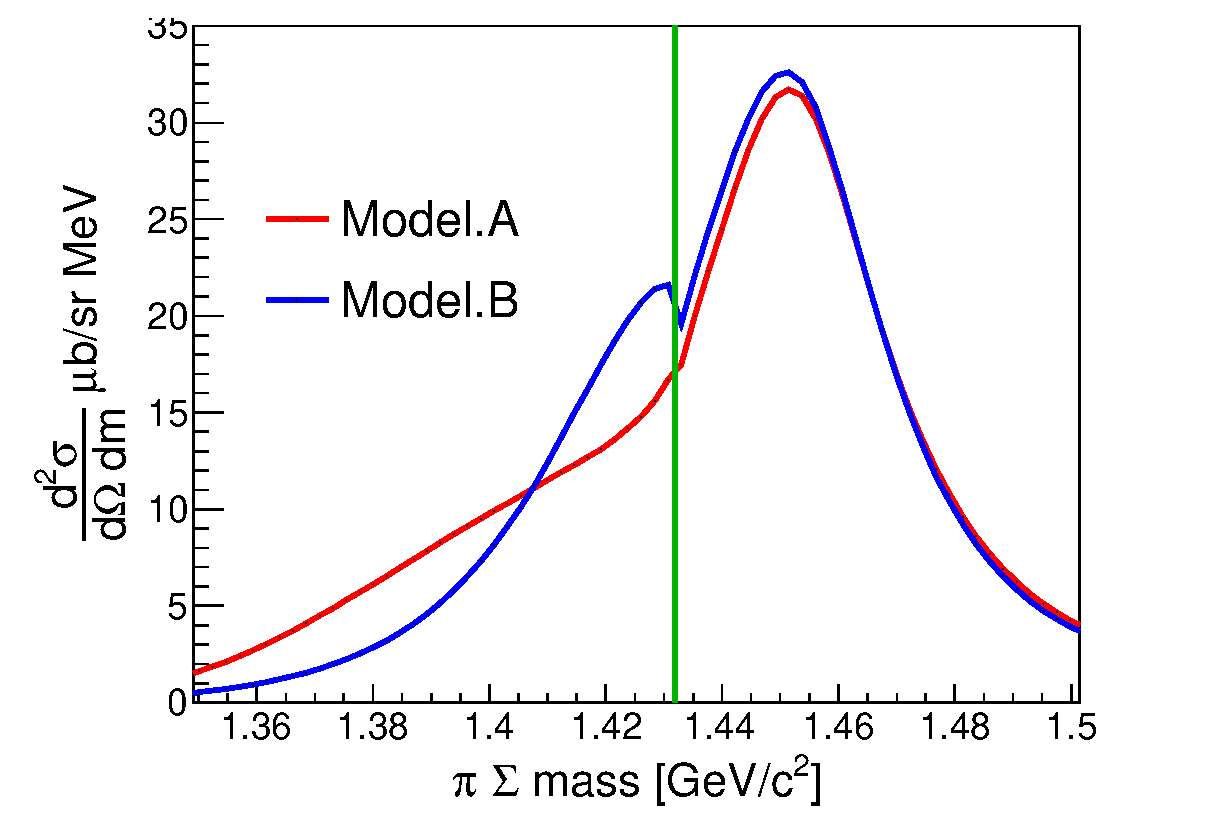
\includegraphics[width=6.0cm]{../pic/Dron/discussion/DCC_pimSp.eps}
    \end{minipage}
    
    \begin{minipage}{0.5\hsize}
      \centering
      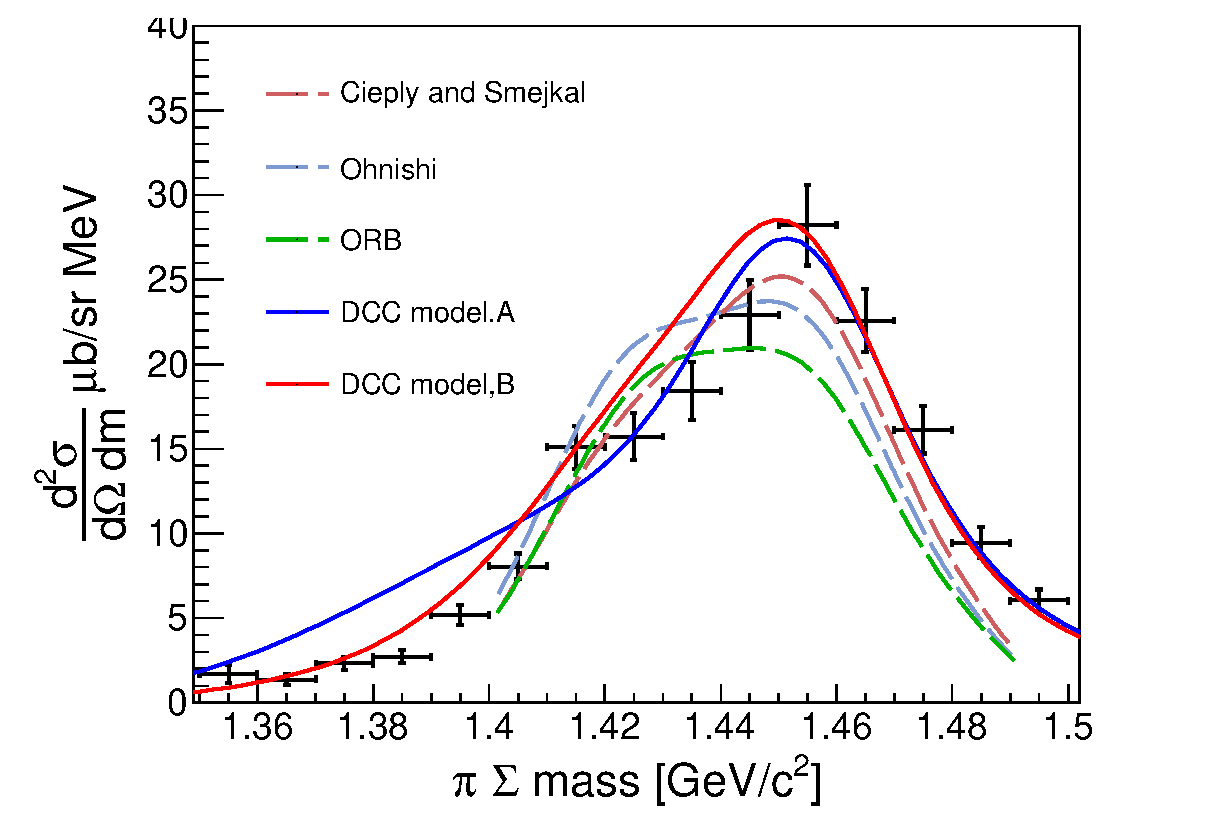
\includegraphics[width=6.0cm]{../pic/Dron/discussion/miyagawa_pimSp.eps}
    \end{minipage}
  \end{tabular}

  \begin{tabular}{cc}
    \begin{minipage}{0.5\hsize}
      \centering
      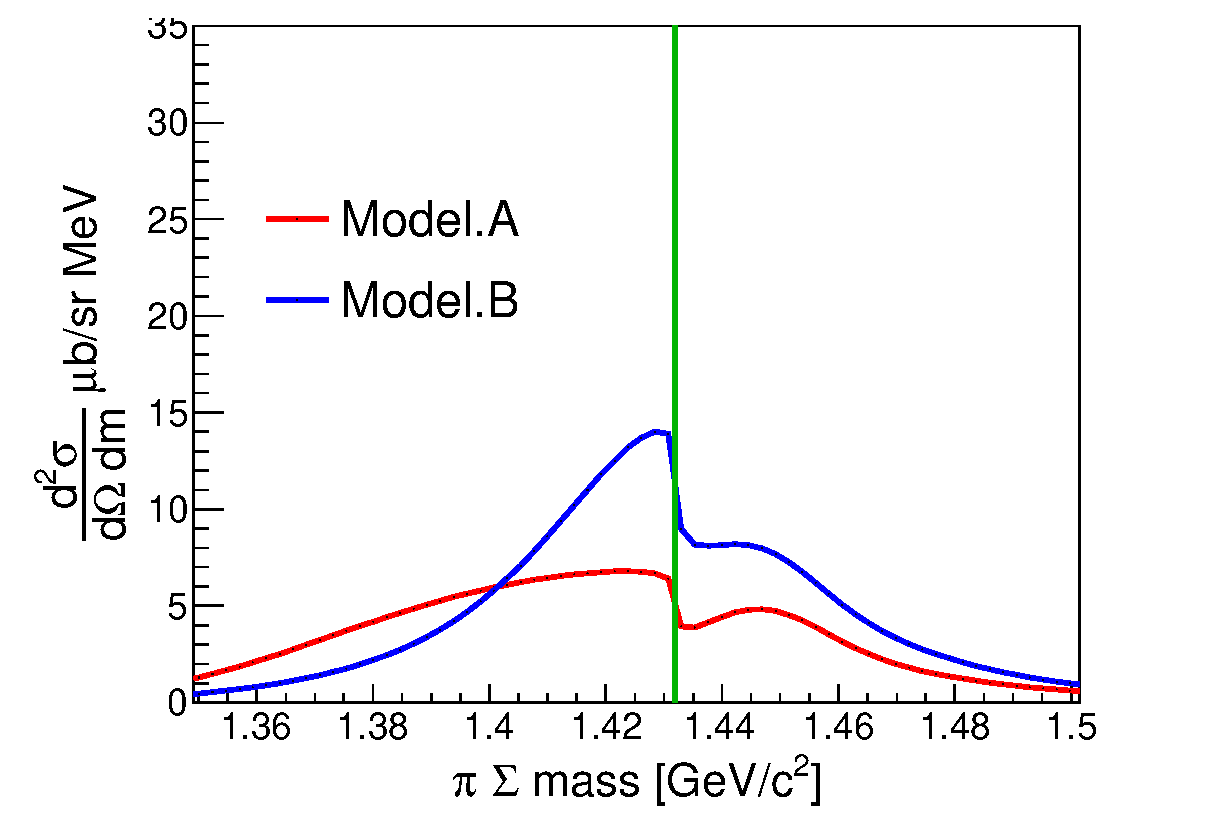
\includegraphics[width=6.0cm]{../pic/Dron/discussion/DCC_pipSm.eps}
    \end{minipage}
    
    \begin{minipage}{0.5\hsize}
      \centering
      \includegraphics[width=6.0cm]{../pic/Dron/discussion/miyagawa_pipSm.eps}
    \end{minipage}
  \end{tabular}

  \begin{tabular}{cc}
    \begin{minipage}{0.5\hsize}
      \centering
      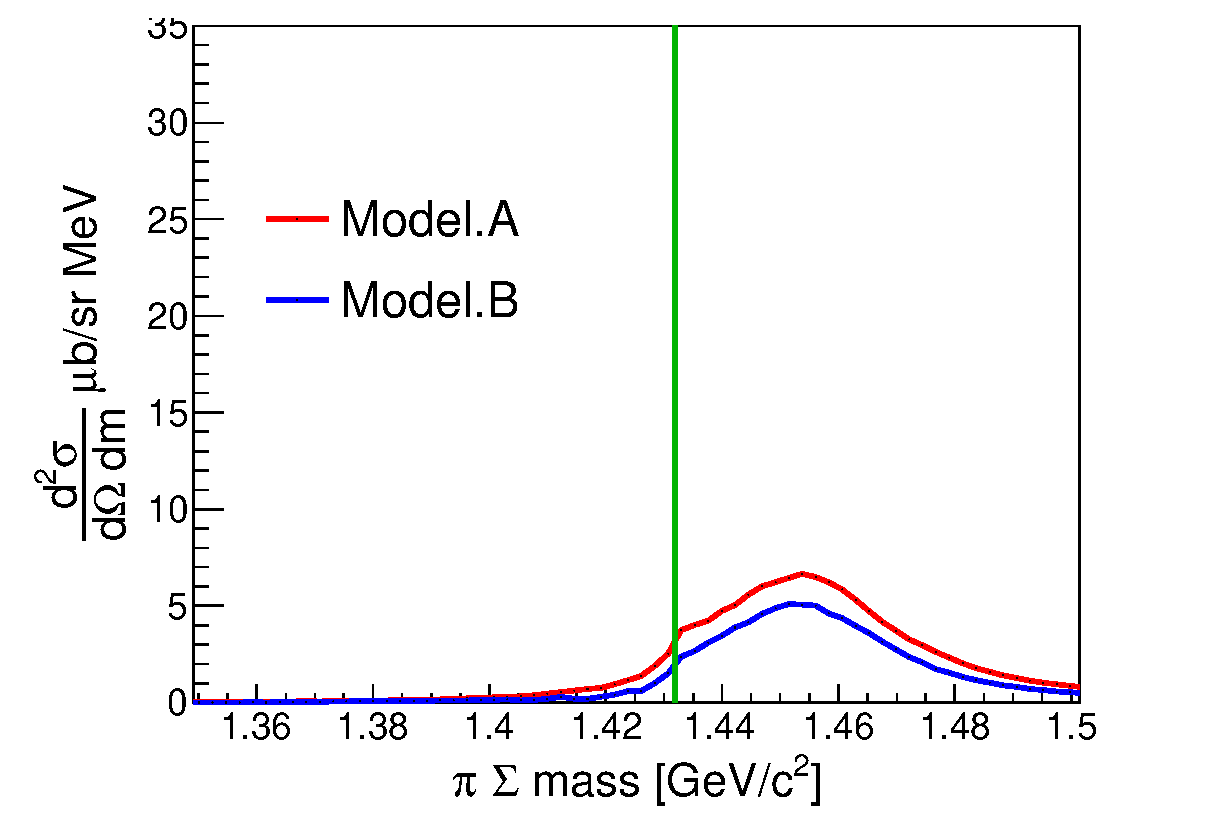
\includegraphics[width=6.0cm]{../pic/Dron/discussion/DCC_pimS0.eps}
    \end{minipage}
    
    \begin{minipage}{0.5\hsize}
      \centering
      \includegraphics[width=6.0cm]{../pic/Dron/discussion/miyagawa_pimS0.eps}
    \end{minipage}
  \end{tabular}
  
  \caption{
    This figure shows a comparison of our obtained spectra with predictions from theoretical calculations.
    The top, middle, and bottom figures represent $\pi^-\Sigma^+$, $\pi^+\Sigma^-$, and $\pi^-\Sigma^0$, respectively.
    The right figure shows the spectrum predicted by the DCC model, and the left figure shows the spectrum predicted by the calculation of Miyagawa et al.
    The spectra predicted by theoretical calculations are convoluted with our detector resolution.
  }
  \label{fig:comp_theoretical_calc}
\end{figure}


The qualitative property of obtained spectra is discussed in the previous subsection.
In this subsection, we discuss the more detail quantitative property by comparing to expected spectra of theoretical calculations.
These theoretical calculations are based on 2-step reaction as described in chapter.1.
This validity is comfirmed in previous subsection.

In the present reaction, the first and second scattering have different kinetic regions.
The first scattering is in the high-energy region with a total energy of 2.05 GeV,
and the $\bar{K}N$ scattering data are abundant in this region and its scattering amplitude is determined with good accuracy.
On the other hand, the second scattering is in the low energy region around the $\bar{K}N$ threshold,
and the $\bar{K}N$ scattering data in this region are not sufficient, especially the scattering amplitude below the $\bar{K}N$ threshold cannot be measured by the elementary process.
One is a method in which the first scattering is calculated using partial wave analysis
and the second scattering is calculated using the results of a low-energy coupled-channels analysis of the $\bar{K}N$ interaction.
One is a method in which the first scattering is calculated using the recent partial wave analysis
and the second scattering is calculated using the results of a 3 different low-energy coupled-channels analysis of the $\bar{K}N$ interaction.
The second one is based on the so-called DCC model, which determines the $\bar{K}N \rightarrow$ meson-baryon scattering amplitudes
from various $\bar{K}N \rightarrow$ meson-baryon scattering data in wide momentum region with meson-baryon interactions based on coupled-channel methods.
Figure.\ref{fig:comp_theoretical_calc} compares the obtained spectra with the theoretical predictions convolved with the experimental resolution.
The upper, middle, and lower panels are shown for $\pi^-\Sigma^+$, $\pi^+\Sigma^-$, and $\pi^0\Sigma^-$, respectively.
The right and left panels show the predictions by the DCC model and the calculations by Miyagawa et al.

The predictions of the DDC model explain the cross sections well for all spectra,
whereas the predictions of Miyagawa et al. cannot explain the obtained spectra due to the lack of overall strength at $\pi^0\Sigma^-$ and the excess of overall strength at $\pi^+\Sigma^-$.
Therefore, in the following, we discuss $I=0$ and $I=1$ and their interference in more detail based on the DCC model.


% In that method, the first scattering is calculated using the results of the partial-wave analysis by the KSU group.
% We employed a two-approach method to compare the obtained spectra with predictions from theoretical calculations.

%% According to this picture, the cross sections have the following relationship,
%% \begin{align}
%%   \frac{d\sigma}{d\Omega dM}(\pi^\mp \Sigma^\pm) & \propto  \left| C^{0}_{1} T_{2}^{I=0} \mp C^{1}_{1} T_{2}^{I=1} \right|^2  & \nonumber \\
%%   & = \left| C^{0}_{1} T_{2}^{I=0} \right|^2 + \left|C^{1}_{1} T_{2}^{I=1} \right|^2 \mp 2\mbox{Re}( C^{0}_{1}C^{1}_{1} T^{I=0}_{2}T^{I=1}_{2} ) & \\
%%   \frac{d\sigma}{d\Omega dM}(\pi^- \Sigma^0) & \propto \left| C^{1}_{1}T_{2}^{I=1} \right|^2 &
%% \end{align}

%% Here, $C_{0}^{1}$ and $C_{1}^{1}$ represents about the scattering factor about first step.
%% So, $C_{1}^{0} = \frac{1}{4\sqrt{3}}\left( 3 T_{1}^{I=0} - T_{1}^{I=1} \right)$ and
%% $C_{1}^{1} = \frac{1}{4}\left( T_{1}^{I=0} + T_{1}^{I=1} \right)$.
%% According to this representation, the factor of $I=0$, $I=1$, and interference term become
%% $\left| C_{1}^{0}T_{2}^{I=0} \right| $, $\left| C_{1}^{1} T_{2}^{I=1} \right|$ and $\mbox{Re}(C^{0}_{1} C^{1}_{1} T^{I=0}_{2} T^{I=1}_{2})$.

